\documentclass[acmtog]{acmart}
\usepackage{graphicx}
\usepackage{subfigure}
\usepackage{natbib}
\usepackage{listings}
\usepackage{bm}
\usepackage{amsmath}

\definecolor{blve}{rgb}{0.3372549 , 0.61176471, 0.83921569}
\definecolor{gr33n}{rgb}{0.29019608, 0.7372549, 0.64705882}
\makeatletter
\lst@InstallKeywords k{class}{classstyle}\slshape{classstyle}{}ld
\makeatother
\lstset{language=C++,
	basicstyle=\ttfamily,
	keywordstyle=\color{blve}\ttfamily,
	stringstyle=\color{red}\ttfamily,
	commentstyle=\color{magenta}\ttfamily,
	morecomment=[l][\color{magenta}]{\#},
	classstyle = \bfseries\color{gr33n}, 
	tabsize=2
}
\lstset{basicstyle=\ttfamily}

\newcommand{\code}[1]{{\color{magenta}{\verb|#1|}}} % for inline code

% Title portion
\title{Assignment 3: {Ray Tracing Basics}} 

\author{Name:\quad hidden  \\ student number:\ hidden
\\email:\quad hidden@shanghaitech.edu.cn}

% Document starts
\begin{document}
\maketitle

\vspace*{2 ex}

\section{Introduction}

In this assignment, the following `must' tasks are completed:
\begin{itemize}
	\item Implement a pin-hole camera model, which is able to shoot optical rays from the camera to the scene.
	\item Implement ray-geometry intersection test, which is able to determine whether a ray intersects with a geometry, including triangle, rectangle and ellipsoid.
	\item Implement light ray sampling with soft shadow, and apply phong lighting model at intersection points.
	\item Implement anti-aliasing using super sampling with rotated grid.
\end{itemize}

And the following `bonus' tasks are done:
\begin{itemize}
	\item Texture mapping.
	\item Normal texture mapping.
	\item Advanced anti-aliasing with the help of Halton sequence.
\end{itemize}

\section{Implementation Details}

\subsection{Camera Model}

The camera model is defined by the following parameters:

\begin{itemize}
	\item Camera position: {\color{magenta}{pos}}.
	\item Camera field of view: {\color{magenta}{fov}}.
	\item Focal length: fixed to $1$ in this assignment.
	\item Forward, Up and Right direction vectors: {\color{magenta}{forward}}, {\color{magenta}{up}} and {\color{magenta}{right}}.
	\item Image resolution and aspect ratio: {\color{magenta}{image}}.
\end{itemize}



Each time the look\_at position or camera position is updated, function {\color{magenta}{Camera::lookAt}} will be called to update `Forward', `Up' and `Right'. \[\begin{cases}
	forward = (look\_at - pos).normalized() \\
	right = (forward \times up).normalized() \\
	up = (right \times forward).normalized()
\end{cases}\]

Then we need to implement the `generate ray' function. We need to generate a ray according to the screen coordinate $(dx, dy)$.

To shoot a ray from the camera to the scene, we need to first determine the position of the pixel on the image plane.
So we calculate the ratio of $d_x$, $d_y$ relatively to the whole image. The leftmost pixel gets x ratio $-1$, rightmost $1$, and the other linearly distributed. The code is:

\begin{lstlisting}
	float ratio_x = (dx / width) * 2 - 1;
	float ratio_y = (dy / height) * 2 - 1;
\end{lstlisting}

Then consider $fov$ and calculate how much the camera needs to biase to the upper and right. The pseudocode is:

\begin{lstlisting}
	float half_up = tan(fov / 2) * focal_len;
	float half_right = half_up * aspect_ratio;
\end{lstlisting}

The ray direction is a normalized vector starting from screen center and pointing to the pixel position. The pseudocode is:

\begin{lstlisting}[language=C++]
	screen_center = cam_pos + forward * focal_len;
	pixel = screen_center
	        + right * ratio_x * half_right
	        + up * ratio_y * half_up;
	ray_dir = (screen_pos - cam_pos).normalized();
\end{lstlisting}

Then we return a ray with the origin at camera position and the direction calculated above.


\subsection{Ray-Geometry Intersection}

We need to determine whether a ray intersects with a geometry, including triangle, rectangle and ellipsoid. The ray-geometry intersection test is implemented in \verb|geometry.cpp|.

\begin{itemize}
	\item \textbf{Ray-triangle intersection}
	
	Suppose the triangle's three vertices are $p_0, p_1, p_2$. Any point inside the triangle can be written as \[
		p(b_1, b_2) = (1-b_1-b_2) p_0 + b_1 p_1 + b_2 p_2	
	\] with conditions $b_1 \geq 0, b_2 \geq 0$ and $b_1 + b_2 \leq 1$.

	To test whether a ray intersects with the triangle, we simply need to solve the following equation: \[
		o + td = (1-b_1-b_2) p_0 + b_1 p_1 + b_2 p_2	
	\]

	The solution of the above equation is \[
		\begin{bmatrix}
			t \\ b_1 \\ b_2
		\end{bmatrix} 
		= 
		\frac{1}{s_1 \cdot e_1}
		\begin{bmatrix}
			s_2 \cdot e_2\\
			s_1 \cdot s\\
			s_2 \cdot e
		\end{bmatrix}
	\] where \[
		\begin{cases}
			e_1 = v_1 - v_0 \\
			e_2 = v_2 - v_0 \\
			s = o - v_0 \\
			s_1 = d \times e_2 \\
			s_2 = s \times e_1
		\end{cases}
	\]

	Check if the $t$, $b_1$ and $b_2$ meets the requirements, and we can determine whether the ray intersects with the triangle.

	\item \textbf{Ray-rectangle intersection}
	
	Suppose the rectangle plane is defined by $(P - P_0)\overrightarrow{n} = 0$.

	To determine intersection, we solve the following equation: \[
		(o + td - P_0) \overrightarrow{n} = 0
	\]

	The solution of $t$ is 
	\[
		t = \frac{\overrightarrow{n} \cdot (P_0 - o)}{\overrightarrow{n} \cdot d}
	\]

	Next, we need to judge whether the point is inside the rectangle. We compute the dot product between $P-P_0$ and the rectangle's `tangent' and `cotangent' (`cotangent' is given by the cross product of `normal' and `tangent'). 

	If the absolute value of the dot product is less than half of the rectangle's width or height, the point is inside the rectangle.


	\item \textbf{Ray-ellipsoid intersection}
	
	Since it would be too complicated to solve the intersection of a ray and an ellipsoid, we first transform the ellipsoid into a unit sphere, solving the intersection with the sphere, and then transform the interaction back. 

	To transform from sphere to ellipsoid, we need the matrix $M$ defined by:
	\[
		T = \begin{bmatrix}
			1 & 0 & 0 & C_x \\
			0 & 1 & 0 & C_y \\
			0 & 0 & 1 & C_z \\
			0 & 0 & 0 & 1
		\end{bmatrix},
		R = \begin{bmatrix}
			a & 0 & 0 & 0 \\
			0 & b & 0 & 0 \\
			0 & 0 & c & 0 \\
			0 & 0 & 0 & 1
		\end{bmatrix},
		S = \begin{bmatrix}
			\|a\| & 0 & 0 & 0 \\
			0 & \|b\| & 0 & 0 \\
			0 & 0 & \|c\| & 0 \\
			0 & 0 & 0 & 1
		\end{bmatrix}
	\]
	and \[
		M = TRS
	\]

	where $C_x, C_y, C_z$ is the center of the sphere, and $a, b, c$ are normalized value. 

	Then we compute the inverse of $M$, $M^{-1}$, and transform the ray from the ellipsoid to the sphere: \[
		\begin{cases}
			o' = M^{-1} o \\
			d' = M^{-1} d
		\end{cases}
	\]

	Then we solve the intersection of the ray and the sphere. The discriminant is given by \[
		\Delta = d' \cdot d' - 4 (o' \cdot d') + 4 (o' \cdot o' - 1)
	\]

	If $\Delta < 0$, there is no intersection. Otherwise, there're one or two intersections, given by \[
		\begin{cases}
			t_1 = \frac{-d' + \sqrt{\Delta}}{2} \\
			t_2 = \frac{-d' - \sqrt{\Delta}}{2}
		\end{cases}
	\]

	We take the smaller one as the intersection point, $\min(t_1, t_2)$, check if it is within $[t_min, t_max]$ range, and transform the intersection point back to the ellipsoid by multipling the matrix $M$: \[
		p = M (o + td)
	\]


\end{itemize}


\subsection{Light Ray Sampling}



In this scene, the light is a square-area light, using rectangle geometry. 

To check if a ray intersects with the light, we simply need to check if the ray intersects with the rectangle, and modify the interaction type to \verb|Light| if it does.

Then we need to sample light rays from the light source to the intersection point. We generate rays using a uniform grid inside the rectangle. The light sample contains the light's color (which is white in this scene), and the sample position inside the area. 

Multiple samples are generated for each light source to allow for soft shadows. We will use \verb|sample_num = 16| to generate $256$ light samples for this scene. 

\begin{center}
	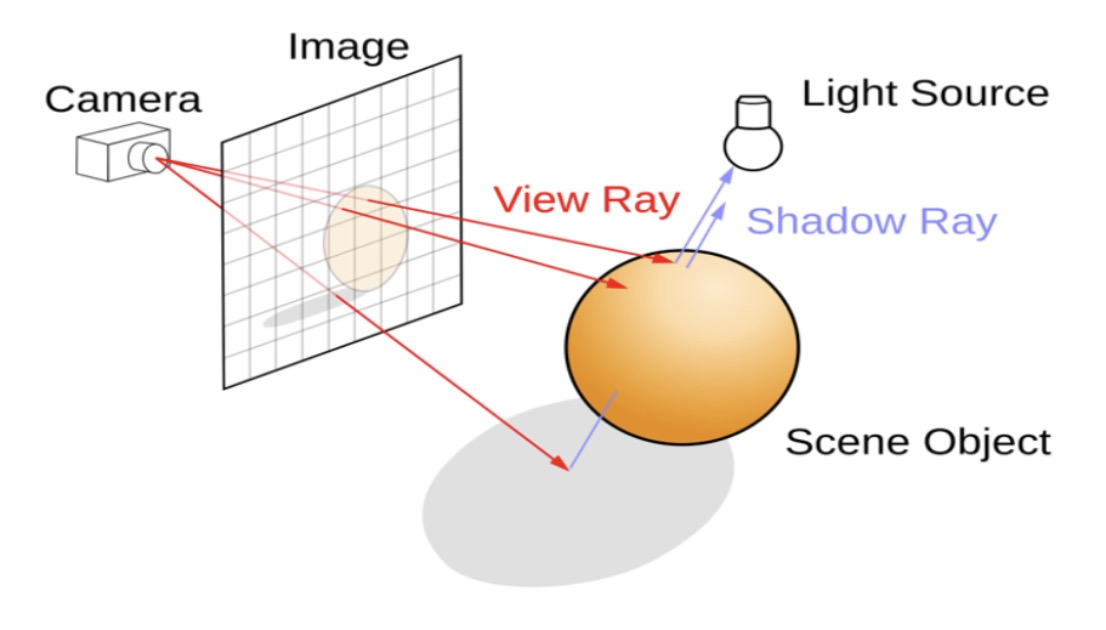
\includegraphics[width=0.4\textwidth]{pictures/phong.jpg}
\end{center}

\subsection{Anti-Aliasing by super sampling}

To reduce aliasing, we need to generate multiple rays in one pixel and take the average color of them. One of the best ways is the rotated grid super sampling. 

\begin{center}
	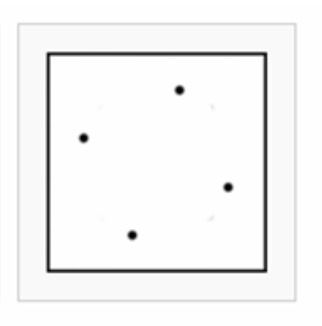
\includegraphics[width=0.2\textwidth]{pictures/rotated-grid.jpg}
\end{center}

Like in the above picture, we generate 4 rays in one pixel rotated an angle of $\arctan(0.5) \approx 26.6°$.

\subsection{Scene intersection and shadowing}

To check if a ray intersects with a scene, we traverse all geometries and check if the ray intersects. We pick the intersection with shortest $t$ value. 

To check whether a ray is shadowed is easier. If a ray has any geometry intersection, it is shadowed. 

\subsection{Texture Mapping}

We will apply texture mapping to rectangle geometry to make the scene more realistic. A texture is a \verb|jpg| image. 

First, we read in the color of each pixel in the texture. We store the pixel color data and the image resolution in \verb|class Texture|. 

Then, in ray-geometry intersection, we need to store \verb|uv| value additionally. In rectangle intersection, after computing the dot product values between $P-P_0$ and the rectangle's `tangent' and `cotangent', we compute the \verb|uv| value by dividing the dot product by the rectangle's width and height. In other words, we compute the ratio of the distance between $P$ and $P_0$ to the rectangle's width and height. The pseudocode is given below:

\begin{lstlisting}[language=C++]
	float dot1 = (p - position).dot(tangent);
	float dot2 = (p - position).dot(cotangent);
	// Process intersection here ...
	float u = clamp01((dot1 / (width / 2) + 1) / 2);
	float v = clamp01((dot2 / (height / 2) + 1) / 2);
\end{lstlisting}

After that, instead of \verb|Const Color Material| that returns a constant phong-lighting-model color, 
we use \verb|Texture Material| that first get the color of the texture at \verb|uv|, and then returns the phong-lighting-model by that color. 
The pixel id is computed by \verb|u * width| and \verb|v * height|.
The shininess value keeps the same, and the remaining process keeps the same. 

In this way, we can see a textured rectangle.

\subsection{Normal Texture Mapping}

In the above section, we applied texture mapping to the rectangle geometry. However, the normal vector of the surface kept the same as the constant value of the rectangle, making it looks completely flat and too smooth. In this section, we will modify the normal value after applying texture mapping to make the surface more realistic.

\begin{center}
	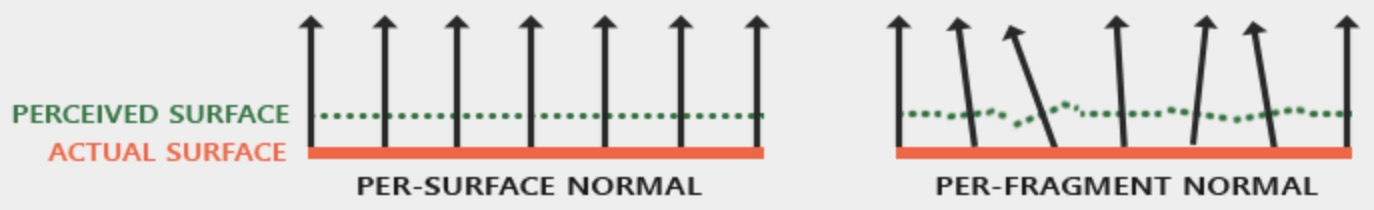
\includegraphics[width=0.45\textwidth]{pictures/normal-texture.jpg}
\end{center}

The normal value of the texture is stored in another picture. However, this is actually not a picture. Its RGB values are representing normal vectors, not colors. The picture have a blue-ish tint because most of the the normals are all closely pointing outwards towards the positive z-axis (0,0,1). 

To apply normal texture mapping, we need to store two textures in the texture material class. One is the color texture, and the other is the normal texture. We also need to add another member function to the texture class, \verb|getNormal(uv)|, to get the normal value of the texture. The value needs to be rounded to $[-1, 1]$, so before it returns the RGB value (in range $[0, 1]$), it multiplies the value by 2 and then subtract 1. The pseudocode is 

\begin{lstlisting}
	Vec3f getNormal(float u, float v) {
		float R, G, B = getColor(u, v);
		return {R * 2 - 1, G * 2 - 1, B * 2 - 1};
	}
\end{lstlisting}

However, this is not the normal we would expect. The normal value is correct only when the rectangle is lying on the ground, facing upwards. Therefore we need to apply a transformation by a 3x3 matrix \verb|TBN|. $T$ means `tangent', $B$ means `bitangent (cotangent)' and $N$ means `normal'. In pseudocode: 

\begin{lstlisting}
// In ray-rectangle intersection ...
interaction.TBN = Mat3(tangent,cotangent,normal);

// In texture evaluation ...
Vec3f normal = texture.getNormal(u, v);
interaction.normal = interaction.TBN * normal;
\end{lstlisting}

In this ray, we can have a normal texture at almost no additional cost, since other than the normal vector, nothing else (including intersection calculation, phong lighting model) are changed.

\subsection{Advanced Anti-Aliasing by Halton Sequence}

In this section, we will apply anti-aliasing by halton sequence.
The halton sequence is a sequence of points with low discrepancy, that is, looks as if it is randomly distributed in the unit square. The halton sequence is generated by the following formula:

\begin{equation}
	h_i = \sum_{j=1}^i \frac{1}{p^j} \bmod 1
\end{equation}

where $p$ is a prime number, and $i$ is the index of the point. The halton sequence is generated by the following pseudocode:

\begin{lstlisting}
float halton(int index, int base) {
	float result = 0;
	float f = 1.0f / base;
	int i = index;
	while (i > 0) {
		result = result + f * (i % base);
		i = floor(i / base);
		f = f / base;
	}
	return result;
}
\end{lstlisting}

In this way, we can generate a sequence of points distributed in a unit square. We can use these points to generate rays and sample the pixels in the image. Since a pixel may have multiple ray samples, the pixel color is the average of them. The pseudocode is given below:

\begin{lstlisting}
for (int i = 0; i < samples; i++) {
	float u = (x + halton(i, 2)) / width;
	float v = (y + halton(i, 3)) / height;
}

// Generate ray and compute color
generateRay(u, v, ray);
color += radiance(ray);
\end{lstlisting}

\newpage

\section{Results}

% \subsection{Rendering result}

% The rendered image of the given scene is below. 

% 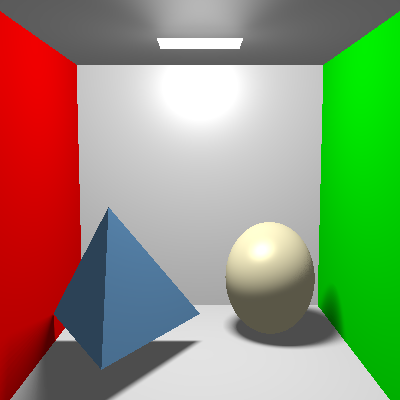
\includegraphics[width=0.2\textwidth]{images/result-ordinary.png}

\subsection{Plain result and Anti-aliasing using super sampling}

The ordinary result, along with the result of anti-aliasing using super sampling, are shown below. In anti-aliasing, we use rotated grid.

\begin{figure}[h]
	\centering
	\subfigure[No antialiasing]
	{
		\begin{minipage}[b]{0.8\linewidth}
			\centering
			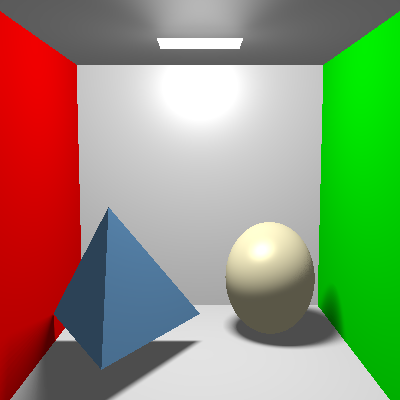
\includegraphics[width=\textwidth]{images/result-ordinary.png}
		\end{minipage}
	}
	\subfigure[With antialiasing]
	{
			\begin{minipage}[b]{0.8\linewidth}
			\centering
			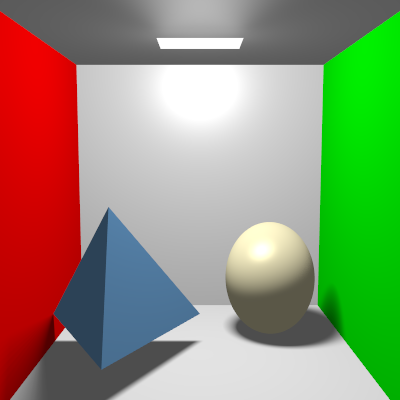
\includegraphics[width=\textwidth]{images/result-antialiasing-4x4.png}
		\end{minipage}
	}
	\caption{Super resolution anti-aliasing}
\end{figure}

\newpage

\subsection{Texture mapping}

We apply texture mapping to the `back wall' and `floor' rectangle geometry. The rendered image is below.

\begin{figure}[h]
	\centering
	\subfigure[Texture mapping]
	{
		\begin{minipage}[b]{0.8\linewidth}
			\centering
			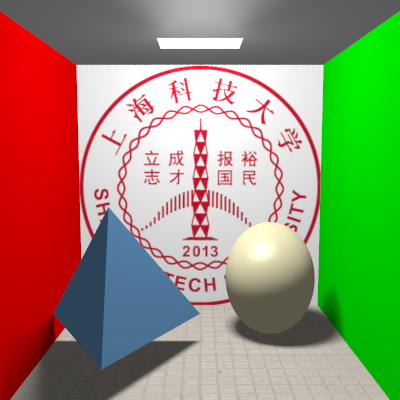
\includegraphics[width=\textwidth]{images/result-texture.png}
		\end{minipage}
	}
	% \caption{Caption}
\end{figure}

\newpage

\subsection{Normal texture mapping}

We apply normal texture mapping to the `back wall' and `floor' rectangle geometry. 

By comparing the image without and with normal texture mapping, we can clearly see that the latter one looks more rough and realistic.

\begin{figure}[h]
	\centering
	\subfigure[Without normal texture]
	{
		\begin{minipage}[b]{0.8\linewidth}
			\centering
			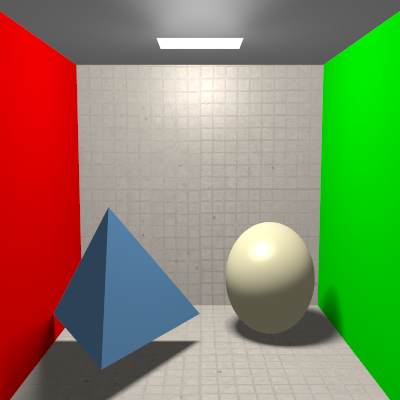
\includegraphics[width=\textwidth]{images/result-without-normal-tex.png}
		\end{minipage}
	}
	\subfigure[With normal texture]
	{
		\begin{minipage}[b]{0.8\linewidth}
			\centering
			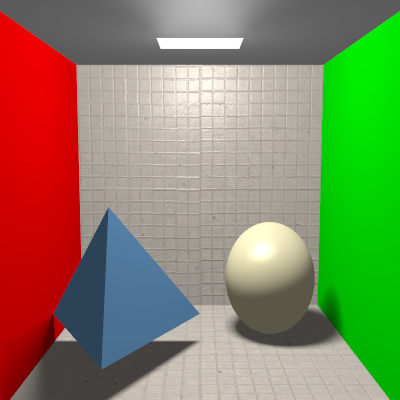
\includegraphics[width=\textwidth]{images/result-with-normal-tex.png}
		\end{minipage}
	}
	\caption{Normal texture mapping}
\end{figure}

\newpage

\subsection{Advanced anti-aliasing by Halton sequence}

We apply advanced anti-aliasing by Halton sequence. The rendered image is below.

\begin{figure}[h]
	\centering
	\subfigure[No antialiasing]
	{
		\begin{minipage}[b]{0.8\linewidth}
			\centering
			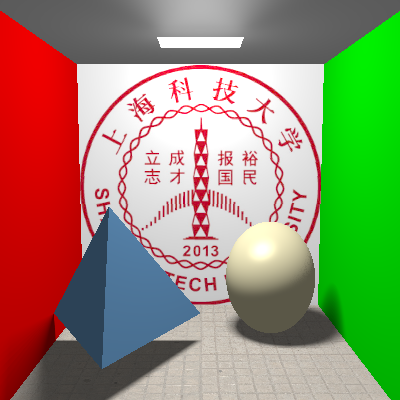
\includegraphics[width=\textwidth]{images/result-no-anti.png}
		\end{minipage}
	}
	\subfigure[Halman sequence anti aliasing]
	{
		\begin{minipage}[b]{0.8\linewidth}
			\centering
			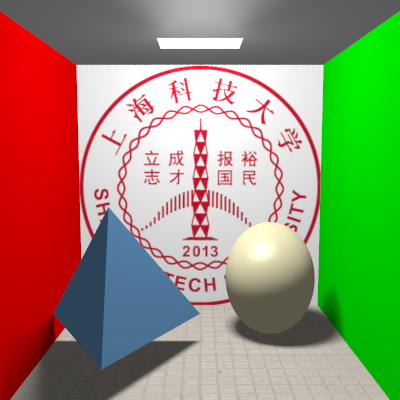
\includegraphics[width=\textwidth]{images/result-halman-seq-antialiasing.png}
		\end{minipage}
	}
	\caption{Advanced antialiasing}
\end{figure}

\end{document}
